%% LyX 2.3.6.1 created this file.  For more info, see http://www.lyx.org/.
%% Do not edit unless you really know what you are doing.
\documentclass[english]{article}
\usepackage[T1]{fontenc}
\usepackage[latin9]{inputenc}
\usepackage{geometry}
\geometry{verbose,tmargin=2.5cm,bmargin=2.5cm,lmargin=2.5cm,rmargin=2.5cm}
\usepackage{graphicx}
\PassOptionsToPackage{normalem}{ulem}
\usepackage{ulem}

\makeatletter

%%%%%%%%%%%%%%%%%%%%%%%%%%%%%% LyX specific LaTeX commands.
%% Because html converters don't know tabularnewline
\providecommand{\tabularnewline}{\\}

\makeatother

\usepackage{babel}
\begin{document}
{[}SPLIT\_HERE{]}
\begin{enumerate}
\item \textbf{{[}HCI/PRELIM/9597/2014/P2/Q1{]} }

Hwa Chong has partnered with Q\&M to set up a dental clinic in the
Campus. The clinic will have a few dentists to serve the student population.
The clinic will also have an on-line system for students to make appointment
with dentist. You are task to design the on-line system to handle
all student appointments. 
\begin{enumerate}
\item Draw an entity-relationship diagram for the appointment system. \hfill{}{[}7{]}
\item Convert the entity-relationship diagram into a relational database
schema. You may use shorthand notation to put across your answers.
Be certain to indicate the key fields. Your solution should include
a brief description for each table. \hfill{}{[}9{]}
\item Ensuring data integrity and security is an important issue in data
design. Explain why they are important for HC Dental system. \hfill{}{[}2{]}
\item The school plans to extent the dental service to other users after
the first year. Modify the entity relationship diagram to cater to
the teachers and staff too. \hfill{}{[}3{]}

Besides the data design, the user interface is an important factor
in determining the success of the HC dental system. The graphical
user interface for students to make an appointment using their desktops/laptops
must be intuitive and usable. 
\item Describe 3 design principles that will guide you in designing your
interfaces. Give specific examples on how you will incorporate it
into your user interface design for the HC dental system. \hfill{}{[}6{]}
\item Design the user-interfaces for the following features 
\begin{enumerate}
\item On-line appointment booking \hfill{}{[}3{]}
\item Updating of students particulars \hfill{}{[}3{]}
\end{enumerate}
\item Part of the future enhancement of the system is to allow a multimodal
interaction between the user and the system. A multimodal human-computer
interaction usually involves the 5 human senses and enables a more
free and natural communication. Suggest 2 realistic possibilities
for such an enhancement. Your suggestions should include a brief description
of how it works in this context.\hfill{}{[}4{]}

HC Dental system will reside in the school server and will allow access
beyond the school intranet. Mr Huang, the network administrator has
allocated an IP address 192.168.123.132 with a subnet mask 255.255.0.0
to access this system. 
\item Explain the following terms: 
\begin{enumerate}
\item IP address \hfill{}{[}1{]}
\item Subnet mask \hfill{}{[}1{]}
\end{enumerate}
\item Based on the information given, what is the network address? Show
the workings. \hfill{}{[}2{]}

The management team is concern with the accuracy of data transmitted/received
outside the school network. To ensure the team that they have looked
into this area, the development team highlighted that they have use
parity checks and checksums in detecting errors 
\item Explain parity checks and give an example to illustrate how it works.
\hfill{}{[}2{]}

The network administrator highlighted that there are proxy and firewalls
settings for devices accessing the school network. 
\item What is the purpose of a proxy server in the Network? \hfill{}{[}2{]}
\end{enumerate}
{[}SPLIT\_HERE{]}
\item \textbf{{[}HCI/PRELIM/9597/2014/P2/Q2{]} }
\begin{enumerate}
\item The Retail Company has engaged a software house to computerize its
operations. The project has been defined to contain the following
list of activities along with their required times for completion:
\noindent \begin{center}
\begin{tabular}{|c|l|c|c|}
\hline 
Activity & Description & Duration (Working Days) & Predecessor/s\tabularnewline
\hline 
\hline 
A & Requirement Analysis & 1 & \tabularnewline
\hline 
B & Systems Design & 3 & A\tabularnewline
\hline 
C & Programming & 5 & B\tabularnewline
\hline 
D & telecoms & 3 & B\tabularnewline
\hline 
E & Hardware Installation & 6 & B\tabularnewline
\hline 
F & Integration & 2 & C, D\tabularnewline
\hline 
G & System Testing & 2 & E, F\tabularnewline
\hline 
H & Training/Support & 1 & G\tabularnewline
\hline 
I & Handover and Go-Live & 1 & H\tabularnewline
\hline 
\end{tabular}
\par\end{center}
\begin{enumerate}
\item Complete the PERT chart below, indicating the earliest start time
and latest start time of each activity: 
\end{enumerate}
\begin{center}
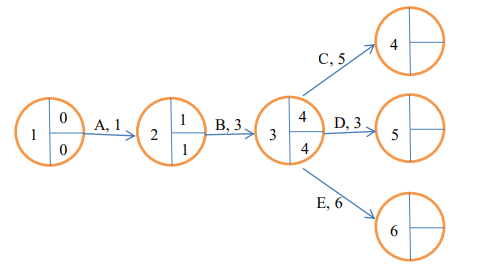
\includegraphics[width=0.65\paperwidth]{C:/Users/Admin/Desktop/Github/question_bank/LyX/static/img/9597-HCI-2014-P1-Q2}
\par\end{center}

\hfill{}{[}4{]}
\begin{enumerate}
\item State the critical path. \hfill{}{[}1{]}
\item State the elapsed time of the project. \hfill{}{[}1{]}
\item State 2 activities not on the critical path, as well as their slack
time. \hfill{}{[}2{]}
\end{enumerate}
\item The Gantt chart below is based on the above information. There are
three activities missing and three activities shown are incorrect.
Draw a sketch of the Gantt chart to show the correct version. 
\noindent \begin{center}
\begin{tabular}{c|c|c|c|c|c|c|c|c|c|c|c|c|c|c|c|c|c|c|c|}
\multicolumn{20}{c}{Weeks}\tabularnewline
\multicolumn{1}{c}{Activity} & \multicolumn{1}{c}{1} & \multicolumn{1}{c}{2} & \multicolumn{1}{c}{3} & \multicolumn{1}{c}{4} & \multicolumn{1}{c}{5} & \multicolumn{1}{c}{6} & \multicolumn{1}{c}{7} & \multicolumn{1}{c}{8} & \multicolumn{1}{c}{10} & \multicolumn{1}{c}{11} & \multicolumn{1}{c}{12} & \multicolumn{1}{c}{13} & \multicolumn{1}{c}{14} & \multicolumn{1}{c}{15} & \multicolumn{1}{c}{16} & \multicolumn{1}{c}{17} & \multicolumn{1}{c}{18} & \multicolumn{1}{c}{19} & \multicolumn{1}{c}{20}\tabularnewline
\cline{2-20} \cline{3-20} \cline{4-20} \cline{5-20} \cline{6-20} \cline{7-20} \cline{8-20} \cline{9-20} \cline{10-20} \cline{11-20} \cline{12-20} \cline{13-20} \cline{14-20} \cline{15-20} \cline{16-20} \cline{17-20} \cline{18-20} \cline{19-20} \cline{20-20} 
A & X &  &  &  &  &  &  &  &  &  &  &  &  &  &  &  &  &  & \tabularnewline
\cline{2-20} \cline{3-20} \cline{4-20} \cline{5-20} \cline{6-20} \cline{7-20} \cline{8-20} \cline{9-20} \cline{10-20} \cline{11-20} \cline{12-20} \cline{13-20} \cline{14-20} \cline{15-20} \cline{16-20} \cline{17-20} \cline{18-20} \cline{19-20} \cline{20-20} 
B &  & X & X & X &  &  &  &  &  &  &  &  &  &  &  &  &  &  & \tabularnewline
\cline{2-20} \cline{3-20} \cline{4-20} \cline{5-20} \cline{6-20} \cline{7-20} \cline{8-20} \cline{9-20} \cline{10-20} \cline{11-20} \cline{12-20} \cline{13-20} \cline{14-20} \cline{15-20} \cline{16-20} \cline{17-20} \cline{18-20} \cline{19-20} \cline{20-20} 
C &  &  &  &  &  & X & X & X & X & X &  &  &  &  &  &  &  &  & \tabularnewline
\cline{2-20} \cline{3-20} \cline{4-20} \cline{5-20} \cline{6-20} \cline{7-20} \cline{8-20} \cline{9-20} \cline{10-20} \cline{11-20} \cline{12-20} \cline{13-20} \cline{14-20} \cline{15-20} \cline{16-20} \cline{17-20} \cline{18-20} \cline{19-20} \cline{20-20} 
D &  &  &  &  &  &  &  & X & X & X &  &  &  &  &  &  &  &  & \tabularnewline
\cline{2-20} \cline{3-20} \cline{4-20} \cline{5-20} \cline{6-20} \cline{7-20} \cline{8-20} \cline{9-20} \cline{10-20} \cline{11-20} \cline{12-20} \cline{13-20} \cline{14-20} \cline{15-20} \cline{16-20} \cline{17-20} \cline{18-20} \cline{19-20} \cline{20-20} 
E &  &  &  &  & X & X & X & X & X & X &  &  &  &  &  &  &  &  & \tabularnewline
\cline{2-20} \cline{3-20} \cline{4-20} \cline{5-20} \cline{6-20} \cline{7-20} \cline{8-20} \cline{9-20} \cline{10-20} \cline{11-20} \cline{12-20} \cline{13-20} \cline{14-20} \cline{15-20} \cline{16-20} \cline{17-20} \cline{18-20} \cline{19-20} \cline{20-20} 
F &  &  &  &  &  &  &  &  &  &  & X & X &  &  &  &  &  &  & \tabularnewline
\cline{2-20} \cline{3-20} \cline{4-20} \cline{5-20} \cline{6-20} \cline{7-20} \cline{8-20} \cline{9-20} \cline{10-20} \cline{11-20} \cline{12-20} \cline{13-20} \cline{14-20} \cline{15-20} \cline{16-20} \cline{17-20} \cline{18-20} \cline{19-20} \cline{20-20} 
G &  &  &  &  &  &  &  &  &  &  &  &  &  &  &  &  &  &  & \tabularnewline
\cline{2-20} \cline{3-20} \cline{4-20} \cline{5-20} \cline{6-20} \cline{7-20} \cline{8-20} \cline{9-20} \cline{10-20} \cline{11-20} \cline{12-20} \cline{13-20} \cline{14-20} \cline{15-20} \cline{16-20} \cline{17-20} \cline{18-20} \cline{19-20} \cline{20-20} 
H &  &  &  &  &  &  &  &  &  &  &  &  &  &  &  &  &  &  & \tabularnewline
\cline{2-20} \cline{3-20} \cline{4-20} \cline{5-20} \cline{6-20} \cline{7-20} \cline{8-20} \cline{9-20} \cline{10-20} \cline{11-20} \cline{12-20} \cline{13-20} \cline{14-20} \cline{15-20} \cline{16-20} \cline{17-20} \cline{18-20} \cline{19-20} \cline{20-20} 
I &  &  &  &  &  &  &  &  &  &  &  &  &  &  &  &  &  &  & \tabularnewline
\cline{2-20} \cline{3-20} \cline{4-20} \cline{5-20} \cline{6-20} \cline{7-20} \cline{8-20} \cline{9-20} \cline{10-20} \cline{11-20} \cline{12-20} \cline{13-20} \cline{14-20} \cline{15-20} \cline{16-20} \cline{17-20} \cline{18-20} \cline{19-20} \cline{20-20} 
\end{tabular}
\par\end{center}

\end{enumerate}
{[}SPLIT\_HERE{]}
\item \textbf{{[}HCI/PRELIM/9597/2014/P2/Q3{]} }

All\textquoteright s Well Hospital is in the process of computerizing
its clinic processes. At the clinic, there are various doctors specializing
in different areas e.g. neuroscience specialists, gynaecologists,
etc. All patients of the clinic must be registered in the patient
database and make prior appointments to see the relevant doctors.
No walk-in patients will be entertained. Appointments are made based
on the doctor\textquoteright s weekly schedule i.e. different doctors
have clinic sessions at different day/time of the week. 

On the day of appointment, patients are to register at the self-registration
counter before proceeding to the doctor\textquoteright s room. Upon
seeing the doctor, the doctor will input the diagnosis into the system.
After the doctor\textquoteright s consultation, the patient is to
proceed to make payment. Upon payment, a prescription slip, reference
letter, medical certificate, will be printed as necessary for the
patient. In addition, the next appointment may be scheduled, if necessary. 
\begin{enumerate}
\item Use a diagram to show the data flows, processes, data stores and external
links in the system. \hfill{}{[}10{]}
\item At the self-registration counter, patients can scan the barcode of
their appointment card or NRIC. Alternatively, they can also enter
their NRIC number using the keyboard. When the NRIC is entered using
the keyboard, it must be validated and verified. 
\begin{enumerate}
\item Explain the difference between validation and verification of data.
\hfill{}{[}2{]}
\item Describe two validation tests that can be performed on the NRIC number
entered. \hfill{}{[}2{]}
\item Describe how the NRIC number entered by the patient can be verified
by the system.\hfill{}{[}1{]}
\end{enumerate}
\item As part of the hospital welfare program, there is a fitness center
for staff. To enter the fitness center, staff needs to use a swipe
card together with a 4-digit PIN to gain access. Access is only allowed
if there are fewer than 50 people already in the fitness center, in
order to avoid overcrowding. Access is also restricted to one person
per card. If maintenance is being carried out then access is denied
and a message is output to a screen asking the staff to return in
1 hour. In order to exit the fitness center, the swipe card is used
again. Using appropriate variable names, write in pseudocode, an algorithm
to control the entry system to the fitness center.\hfill{}{[}8{]}
\end{enumerate}
{[}SPLIT\_HERE{]}
\item \textbf{{[}HCI/PRELIM/9597/2014/P2/Q4{]} }

A Retail Company has a customer loyalty program that gives a range
of discounts. For customers in the loyalty program between 5 to 9
years, they will receive a 5\% discount. For 10 or more years, the
customer will receive a 10\% discount. However, whether a customer
is in the loyalty program or not, if the cumulative value of his purchases
for this calendar year exceed \$1000, he will receive a 15\% discount.
Note: Aggregation of discounts is not allowed. 
\begin{enumerate}
\item Create a decision table that shows all possible outcomes for the above
loyalty program. 
\item Draw the decision table after redundancies have been removed. \hfill{}{[}6{]}
\item Using your answer in (b), write a function using pseudocode. The function
returns: 
\begin{itemize}
\item 0 to indicate no discount 
\item the percentage discount offered\hfill{}{[}4{]}
\end{itemize}
\end{enumerate}
{[}SPLIT\_HERE{]}
\item \textbf{{[}HCI/PRELIM/9597/2014/P2/Q5{]} }

An apartment block in a city consists of a large number of apartments.
Each of the residents of the apartments has their information stored
in a file. 

The records in the file are to be sorted into alphabetical order of
the resident\textquoteright s name. 
\begin{enumerate}
\item Using the following list of names as an example, show how the records
can be sorted into alphabetical order using an insertion sort. 
\noindent \begin{center}
GRA, CHR, DAV, SAR, TOM, KAT \hfill{}{[}4{]}
\par\end{center}
\item Residents sometimes make requests for maintenance on their apartments.
Each request is given a priority number ranging from 1, for failure
of the air conditioning, to 10, for a dripping tap. Each request is
stored in a linked list in order of priorities. Jobs with equal priority
are stored in order of the date that they have been submitted. 

Describe an algorithm to insert a new job into the list. \hfill{}{[}6{]}
\end{enumerate}
{[}SPLIT\_HERE{]}
\item \textbf{{[}HCI/PRELIM/9597/2014/P1/Q1{]} }

A program is to process daily high scores recorded from an online
game. The program can be run every day. 

All scores are integers in the range 1 to 500.

The program reads from file \texttt{HIGHEST.txt} the current highest
score and player name from running the program on previous days. 

The program specification is to: 
\begin{itemize}
\item input up to 5 player names and their corresponding scores for today 
\item calculate and display on screen: 
\begin{itemize}
\item the highest score with the player name for today 
\item a message saying whether or not the highest score today beat the current
highest score 
\end{itemize}
\item update the file \texttt{HIGHEST.txt} if a higher score was input today. 
\end{itemize}

\subsection*{Task 1.1 }

Write program code for this task. 

\subsection*{Evidence 1: }

Your program code. \hfill{}{[}7{]}

\subsection*{Task 1.2 }

Draw up a set of test data which tests the functioning of your program.
Consider carefully all cases which could occur for both the scores
input and the two processing requirements. 

\subsection*{Evidence 2: }

A screenshot for each test case you considered. Annotate the screenshot
explaining the purpose of each test. \hfill{}{[}8{]}

A \textbf{\emph{palindrome}} is an integer that reads the same backwards
and forwards -{}- so 6, 11 and 121 are all palindromes, while 10,
12, 223 and 2244 are not (even though 010=10, we don't consider leading
zeroes when determining whether a number is a palindrome). 

\subsection*{Task 1.3 }

Write program code with the following specification: 
\begin{itemize}
\item input two integers -{}- the endpoints of an interval e.g. \texttt{10
120 }
\item output the number of integers that are palindromes in the interval. 
\end{itemize}

\subsection*{Evidence 3: }

Your program code. \hfill{}{[}8{]}

\subsection*{Evidence 4: }

Produce two screenshots showing the output of 1 4 and 10 120 by the
user.\hfill{} {[}2{]}

{[}SPLIT\_HERE{]}
\item \textbf{{[}HCI/PRELIM/9597/2014/P1/Q2{]} }

The following is a pseudocode algorithm for the quick sort function. 

The function takes in an array and returns a sorted array in \textbf{ascending}
order. The algorithm works for most input but is missing out on a
few edge cases. 

\noindent %
\noindent\begin{minipage}[t]{1\columnwidth}%
\texttt{FUNCTION quicksort(array) }

\texttt{\qquad{}if array length = 1 }

\texttt{\qquad{}\qquad{}return array }

\texttt{\qquad{}select and remove a pivot value from array }

\texttt{\qquad{}create empty subarrays less and greater }

\texttt{\qquad{}for each item in array}

\texttt{\qquad{}\qquad{}if item < pivot }

\texttt{\qquad{}\qquad{}\qquad{}append item to less }

\texttt{\qquad{}\qquad{}else }

\texttt{\qquad{}\qquad{}\qquad{}append item to greater}

\texttt{\qquad{}return quicksort(less) + pivot + quicksort(greater) }%
\end{minipage}

\subsection*{Task 2.1 }

Write program code for this algorithm including all the amendments
you would make to: 
\begin{itemize}
\item make the function work for all cases 
\item adhere to good programming style 
\end{itemize}
Use the \texttt{Team} array sample data available from text file \texttt{SPORT+NAME+TEAM.txt}
and paste this into your program code.

\subsection*{Evidence 5: }

Your program code.\hfill{} {[}6{]}

\subsection*{Evidence 6: }

One screenshot showing the output from running the program code for
array Team.\hfill{} {[}1{]}

The following is a pseudocode algorithm of a binary search written
by a student to search for an item in an array Sport. This array stores
string data arranged in ascending order and has a final subscript
MAX. 

The algorithm is poorly designed and also contains errors. 

\noindent %
\noindent\begin{minipage}[t]{1\columnwidth}%
\texttt{Enter k }

\texttt{A = 1 }

\texttt{B = MAX }

\texttt{While not found }

\texttt{\qquad{}C = (A+B) DIV 2 }

\texttt{\qquad{}If Sport(C) = k }

\texttt{\qquad{}\qquad{}Print \textquotedblleft Found\textquotedblright{} }

\texttt{\qquad{}Else If Sport(C) < k }

\texttt{\qquad{}\qquad{}B = C-1 }

\texttt{\qquad{}Else }

\texttt{\qquad{}\qquad{}A = C+1 }

\texttt{\qquad{}End-If-Else }

\texttt{End-While }%
\end{minipage}

\subsection*{Task 2.2 }

Write program code for this algorithm including all the changes you
would make to: 
\begin{itemize}
\item follow good programming practice 
\item make the algorithm work properly 
\end{itemize}
Use the sample array data available from text file \texttt{SPORT+NAME+TEAM.txt}
and paste this into your programming code. 

\subsection*{Evidence 7: }

Your program code. \hfill{}{[}7{]}

\subsection*{Task 2.3 }

The binary search code could be useful for many programs where a search
routine is required. 

Re-design the program code to have a procedure \texttt{BinarySearch}.
This procedure should have parameters which allow it to be used for
\uline{any} sorted array of string data. 

Use the data provided in the array \texttt{Name} from text file \texttt{SPORT+NAME+TEAM.txt}
and test the procedure with appropriate test cases to ensure it is
working properly. 

\subsection*{Evidence 8: }

Your amended program code. \hfill{}{[}3{]}

\subsection*{Evidence 9: }

A screenshot for each appropriate test case. \hfill{}{[}3{]}

{[}SPLIT\_HERE{]}
\item \textbf{{[}HCI/PRELIM/9597/2014/P1/Q3{]} }

Morse Code is a type of code in which letters are represented by combinations
by long or short signals, e.g. the letter \textquoteleft A\textquoteright{}
is represented by a short followed by a long signal, i.e. \textquoteleft .-\textquoteleft{} 

Here we use the period (\textquoteleft .\textquoteright ) to represent
the short signal and the dash (\textquoteleft -\textquoteleft ) to
present the long signal. The Morse code equivalent for the letters
\textquoteleft A\textquoteright{} to \textquoteleft Z\textquoteright{}
is provided in the file \texttt{MORSE.txt}. In this implementation,
we use a space (\textquoteleft{} \textquoteleft ) to simulate the
inter-character gap and the slash (\textquoteleft /\textquoteright )
to represent the inter-word gap. 

\subsection*{Task 3.1 }

Write the program code for a function that will convert a given word
into its Morse Code equivalent using the following specification. 
\noindent \begin{center}
\texttt{FUNCTION ConvertWord(SingleWord : STRING): STRING }
\par\end{center}

The function has a single parameter \texttt{SingleWord} and returns
the Morse Code equivalent for that word as a string. 

\subsection*{Evidence 10: }

Your \texttt{ConvertWord} program code. \hfill{} {[}7{]}

\subsection*{Evidence 11: }

A screenshot showing the correct Morse Code equivalent for the word
\textquotedblleft COMPUTING\textquotedblright . \hfill{} {[}1{]}

\subsection*{Task 3.2 }

Write the program code that does the following: 
\begin{itemize}
\item the user inputs a sentence of words not exceeding 5 words. 
\item uses the function \texttt{ConvertWord} in Task 3.1 
\item outputs the Morse Code equivalent of the sentence of words that was
entered. 
\end{itemize}

\subsection*{Evidence 12: }

Your program code. \hfill{} {[}6{]}

\subsection*{Task 3.3}

Draw up \textbf{two} suitable tests to assess that your program is
working properly, explaining the reason for each test and provide
screenshot evidence for your testing. 

\subsection*{Evidence 13: }

Annotated screenshots for each test data run. \hfill{} {[}4{]}

\subsection*{Task 3.4 }

Write the program code that will do the following: the user enters
a word string in Morse Code the program converts the Morse Code word
to its alphabetical equivalent outputs the converted word.

\subsection*{Evidence 14: }

Your program code. \hfill{}{[}6{]}

\subsection*{Evidence 15: }

A screenshot showing the correct word equivalent for the following
Morse Code string, \textquotedblleft \dots{} \texttt{-{}-{}-} \dots \textquotedblright{}
\hfill{}{[}1{]}

{[}SPLIT\_HERE{]}
\item \textbf{{[}HCI/PRELIM/9597/2014/P1/Q4{]} }

Many programming languages use a variety of brackets eg \texttt{()},
\texttt{\{\}} and \texttt{{[}{]}} in their program statement constructs.
Brackets can be nested e.g. (()) and \{{[}{]}\}. A well-formed construct
must contain a matched set of optionally nested brackets e.g.\texttt{ (())},
\texttt{\{{[}{]}\}} and \texttt{()\{\}{[}{]}} are well-formed whereas\texttt{
(()},\texttt{ \{{]} }and\texttt{ )( }are not. 

An efficient way to check if a program construct is well-formed is
to use a stack to scan the brackets once from left to right as follows: 

Start from an empty stack. Whenever we encounter an open bracket,
push it into the stack. Whenever we encounter a close bracket, we
check if it is of the same type with the item at the top of the stack.
Once we have a match, we pop the topmost bracket from the stack. Only
when we managed to read the last bracket and find that the stack is
empty, then we know that the brackets are properly nested, and the
program construct is well-formed. 

The stack ADT contains character data and a top pointer, and has the
following operations: 
\begin{itemize}
\item \texttt{Create()} : initializes a new stack 
\item \texttt{Push(item)} : add item to top of stack 
\item \texttt{Pop()} : remove item from top of stack 
\item \texttt{Peep()} : inspect the topmost item of stack 
\item \texttt{isEmpty()} : check if stack is empty 
\end{itemize}

\subsection*{Task 4.1 }

Using object-oriented programming techniques, implement the stack
ADT using the class name \texttt{Stack}. 

\subsection*{Evidence 16: }

Your \texttt{Stack} class program code. \hfill{}{[}8{]}

\subsection*{Task 4.2 }

Write a function \texttt{CheckNested(construct)} which accepts a string
program construct of nested brackets and returns a Boolean result
indicating if construct is well-formed. 

\subsection*{Evidence 17: }

Your \texttt{CheckNested} function code. \hfill{}{[}10{]}

\subsection*{Task 4.3}

Test your \texttt{CheckNested} function using the data file provided
in \texttt{DATA.txt}. If a construct is not well-formed, append it
to a text file \texttt{ERRORS.txt}. 

\subsection*{Evidence 18: }

Screenshot of \texttt{ERRORS.txt}. \hfill{}{[}1{]}

\subsection*{Task 4.4}

Write a function \texttt{CheckWellformed(construct)} which contains
a modified and enhanced version of \texttt{CheckNested(construct)}.
When a first mismatch of bracket occurs, output the diagnostic message
\texttt{\textquotedbl Expecting '?'\textquotedbl}, where ? is the
type of bracket expected. For example, for the construct \texttt{())},
output the diagnostic message \texttt{\textquotedbl Expecting '('\textquotedbl}. 

\subsection*{Evidence 19: }

Your \texttt{CheckWellformed} function code. \hfill{}{[}10{]}

\subsection*{Task 4.5}

Test your \texttt{CheckWellformed} function using \texttt{ERRORS.txt}.
Display the diagnostic messages to screen.

\subsection*{Evidence 20: }

Screenshot of diagnostic messages on screen. \hfill{}{[}1{]}

{[}SPLIT\_HERE{]}
\end{enumerate}
 
\end{document}
